\begin{landscape}
\section{Extension Task Inputs and Outputs}
\label{sec:extension-task-data}

Table~\ref{tab:agent-contracts} records the natural-language contracts and
representative observable inputs and outputs for the 12 tasks used in the
agent and footprint experiments.  Tables~\ref{tab:extension-type}--\ref{tab:extension-layout} specify construction,
verification, and print/parse round trips. Rejected inputs produce no output IR.
Tensor types omit the \texttt{tensor<\ldots{}>} wrapper; bare i8 or f32 denotes a
rank-zero tensor. Axis indices are zero-based.

\scriptsize
\setlength{\tabcolsep}{3pt}
\renewcommand{\arraystretch}{1.12}
\begin{longtable}{@{}p{1.2cm}p{2.5cm}p{6.8cm}p{5.0cm}p{4.5cm}@{}}
\caption{Natural-language task contracts and representative observable inputs
and outputs.  The table preserves the operative semantic constraints while
omitting only system-specific entry-point boilerplate.  Every candidate is
also checked on disjoint hidden cases.}
\label{tab:agent-contracts}\\
\toprule
Family & Task & Natural-language request & Positive input $\rightarrow$ output & Boundary or negative input $\rightarrow$ observation \\
\midrule
\endfirsthead
\multicolumn{5}{l}{\textit{Table~\ref{tab:agent-contracts} continued}}\\
\toprule
Family & Task & Natural-language request & Positive input $\rightarrow$ output & Boundary or negative input $\rightarrow$ observation \\
\midrule
\endhead
\midrule
\multicolumn{5}{r}{\textit{continued on next page}}\\
\endfoot
\bottomrule
\endlastfoot

Definition & \texttt{def-parametric-type} &
Define a signed fixed-point scalar \texttt{fx<W,F>}; require $2\leq W\leq32$
and $0\leq F<W$.  Preserve both parameters through construction, printing,
and reparsing; native function arguments and returns use the new type. &
\texttt{type=fx, W=8, F=3} $\rightarrow$ \texttt{fx<8,3>}, logical width 8 &
\texttt{W=8, F=8} $\rightarrow$ \texttt{invalid-type-parameter} during typing; no output IR \\

Definition & \texttt{def-quantized-op} &
Define \texttt{qadd} on equal-shape i8 tensors.  Input and output scales are
finite and positive; zero points are signed i32.  The result preserves the
operand shape and i8 element type. &
two \texttt{tensor<4xi8>} operands, scales 0.5/0.25/0.5, zeros 0/$-3$/0
$\rightarrow$ \texttt{tensor<4xi8>} &
\texttt{2x3xi8} plus \texttt{3x2xi8} $\rightarrow$ \texttt{shape-mismatch} \\

Analysis & \texttt{ana-broadcast-shape} &
Analyze NumPy trailing-dimension broadcasting for nonnegative extents.  Pad
the shorter shape with leading ones; aligned extents must be equal or one,
and a one selects the other extent, including zero. &
\texttt{[2,3,1]}, \texttt{[4]} $\rightarrow$ legal, \texttt{[2,3,4]} &
\texttt{[2,3]}, \texttt{[4,3]} $\rightarrow$ illegal, conflict axis 1 from the end \\

Analysis & \texttt{ana-numeric-range} &
Propagate closed finite intervals through add, multiply, ReLU, and clamp;
multiplication evaluates all four endpoint products. &
\texttt{mul([-2,3],[-4,5])} $\rightarrow$ \texttt{[-12,15]} &
\texttt{relu([2,-1])} $\rightarrow$ \texttt{invalid-interval} \\

Rewrite & \texttt{rew-add-zero} &
Replace integer add-by-zero when type and shape are preserved.  Floating
positive zero additionally requires \texttt{no\_signed\_zeros}; retain
negative zero.  Remove a matched constant only when it has no remaining uses. &
f32 \texttt{x+0}, shape \texttt{[4]}, \texttt{no\_signed\_zeros=true}
$\rightarrow$ replace by \texttt{x} &
f32 \texttt{x+0.001} $\rightarrow$ keep operation \\

Rewrite & \texttt{rew-redundant-cast} &
Remove identity casts and cancel round trips only for lossless signed-integer
widening or finite f32-to-f64 widening.  Keep narrowing, float--integer, and
shape-changing conversions. &
\texttt{f32[4] -> f32[4]} $\rightarrow$ eliminate cast &
\texttt{i16[4] -> i8[4] -> i16[4]} $\rightarrow$ retain casts \\

Conversion & \texttt{con-gelu-expand} &
Replace native SSA \texttt{gelu} by
$0.5x(1+\operatorname{erf}(x/\sqrt{2}))$ using declared primitive targets.
Preserve shape, floating element type, and every output user. &
\makebox[\linewidth][c]{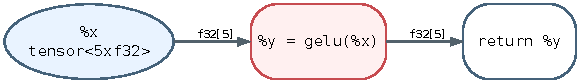
\includegraphics[width=0.92\linewidth]{figures/agent-gelu-before.pdf}}\par
\texttt{gelu}, f32, shape \texttt{[5]} &
\makebox[\linewidth][c]{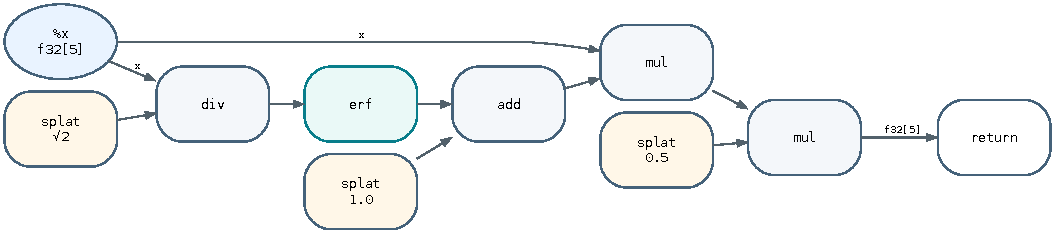
\includegraphics[width=0.92\linewidth]{figures/agent-gelu-after.pdf}}\par
no \texttt{gelu}; graph contains \texttt{erf}. Integer input
$\rightarrow$ \texttt{unsupported-element-type}; no output IR \\

Conversion & \texttt{con-quant-expand} &
Convert i8 tensor \texttt{qadd} into two dequantizations, f32 add, and
quantization with ties-to-even rounding and i8 saturation.  Preserve shape
and result users. &
\texttt{[-3,0,5,120]} plus \texttt{[2,1,-8,120]}, scale 0.5
$\rightarrow$ \texttt{[-1,1,-3,127]} &
negative scale $\rightarrow$ \texttt{invalid-scale}; no output IR \\

Emission & \texttt{emit-graph-manifest} &
Emit deterministic schema-v1 JSON from a typed SSA function.  Number nodes
and values in stable order; preserve repeated operands, output order, types,
and sorted user attributes; omit declarations and source names. &
\texttt{splat -> add -> relu} $\rightarrow$ nodes \texttt{n0..n2}, values
\texttt{v0..v3}, output \texttt{v3} &
Repeated emission $\rightarrow$ byte-identical JSON \\

Emission & \texttt{emit-kernel-wrapper} &
Emit a complete C99 translation unit exporting
\texttt{task\_kernel(input,output,count)} for ReLU or $2x+1$.  Support exact
in-place execution and zero count; do not touch guards or nonaliased inputs. &
ReLU on \texttt{[-2,-0,1.5,4]} $\rightarrow$ \texttt{[+0,+0,1.5,4]} &
\texttt{count=0}, null pointers $\rightarrow$ no access; compiled driver and guard oracle pass \\

Vertical & \texttt{vert-int4} &
Add signed qint4 values, saturate to $[-8,7]$, and pack two's-complement
nibbles low-first.  For odd counts, zero the unused high nibble.  Reject
out-of-range source literals before addition. &
\texttt{[-8,-1,0,3,7]} plus \texttt{[1,1,-2,6,7]}
$\rightarrow$ \texttt{[-7,0,-2,7,7]}, bytes \texttt{09 7e 07} &
literal 8 $\rightarrow$ \texttt{literal-out-of-range} \\

Vertical & \texttt{vert-fused-op} &
Add NHWC/HWIO signed-i8 \texttt{fused\_qconv\_relu}: valid unit-stride
cross-correlation, i32 bias, ties-to-even requantization, i8 saturation, and
real-domain ReLU.  Fuse only a single-use qconv--bias--requantize--ReLU chain. &
unit kernel with input \texttt{[1,-2]}, weights \texttt{[2,-3]}, bias 1
$\rightarrow$ \texttt{[4]} and one fused manifest node &
shared convolution result $\rightarrow$ no match; original chain preserved \\

\end{longtable}
\end{landscape}

\subsection{Parametric Type Definition}
\begin{table}[H]
\caption{\texttt{def-parametric-type}: complete inputs and expected outputs.
Width denotes logical bits, not ABI allocation size.}
\label{tab:extension-type}
\centering
\scriptsize
\setlength{\tabcolsep}{3pt}
\begin{tabular*}{\textwidth}{@{\extracolsep{\fill}}llllll@{}}
\toprule
Case & Width & Fraction bits & Expected type & Logical bits & Expected diagnostic \\
\midrule
fx8-3 & 8 & 3 & \texttt{fx<8,3>} & 8 & --- \\
fx16-7 & 16 & 7 & \texttt{fx<16,7>} & 16 & --- \\
minimum-integer & 2 & 0 & \texttt{fx<2,0>} & 2 & --- \\
minimum-fraction & 2 & 1 & \texttt{fx<2,1>} & 2 & --- \\
maximum-integer & 32 & 0 & \texttt{fx<32,0>} & 32 & --- \\
maximum-fraction & 32 & 31 & \texttt{fx<32,31>} & 32 & --- \\
fraction-overflow & 8 & 8 & --- & --- & invalid-type-parameter \\
width-too-small & 1 & 0 & --- & --- & invalid-type-parameter \\
width-too-large & 33 & 0 & --- & --- & invalid-type-parameter \\
negative-width & -2 & 0 & --- & --- & invalid-type-parameter \\
negative-fraction & 8 & -1 & --- & --- & invalid-type-parameter \\
\bottomrule
\end{tabular*}
\end{table}

\subsection{Quantized Operation Definition}
\begin{table}[H]
\caption{\texttt{def-quantized-op}: complete inputs and expected outputs, with
defaults expanded. Scales are finite positive f64 values; zero points are signed
i32 values. This task defines the operation; arithmetic lowering is evaluated separately.}
\label{tab:extension-qadd}
\centering
\scriptsize
\setlength{\tabcolsep}{3pt}
\begin{tabular*}{\textwidth}{@{\extracolsep{\fill}}llllll@{}}
\toprule
Case & LHS type & RHS type & Scales (L, R, out) & Zero points (L, R, out) & Expected result / diagnostic \\
\midrule
vector & 4$\times$i8 & 4$\times$i8 & 0.5, 0.25, 0.5 & 0, -3, 0 & 4$\times$i8 \\
matrix & 2$\times$3$\times$i8 & 2$\times$3$\times$i8 & 0.125, 0.125, 0.25 & 2, 2, 1 & 2$\times$3$\times$i8 \\
scalar & i8 & i8 & 1, 1, 0.25 & 0, 0, 0 & i8 \\
empty-axis & 0$\times$3$\times$i8 & 0$\times$3$\times$i8 & 1, 1, 0.5 & 0, 0, 0 & 0$\times$3$\times$i8 \\
signed-zero-point-bounds & 1$\times$2$\times$3$\times$i8 & 1$\times$2$\times$3$\times$i8 & 0.0625, 2, 1 & $-$2$^{31}$, 2$^{31}$$-$1, $-$2$^{31}$ & 1$\times$2$\times$3$\times$i8 \\
shape-mismatch & 2$\times$3$\times$i8 & 3$\times$2$\times$i8 & 1, 1, 0.5 & 0, 0, 0 & shape-mismatch \\
zero-scale & 4$\times$i8 & 4$\times$i8 & 1, 1, 0 & 0, 0, 0 & invalid-scale \\
lhs-zero-scale & 4$\times$i8 & 4$\times$i8 & 0, 1, 1 & 0, 0, 0 & invalid-scale \\
rhs-negative-scale & 4$\times$i8 & 4$\times$i8 & 1, -0.25, 1 & 0, 0, 0 & invalid-scale \\
negative-output-scale & 4$\times$i8 & 4$\times$i8 & 1, 1, -0.5 & 0, 0, 0 & invalid-scale \\
lhs-element & 4$\times$i16 & 4$\times$i8 & 1, 1, 1 & 0, 0, 0 & operand-type-mismatch \\
rhs-element & 4$\times$i8 & 4$\times$i16 & 1, 1, 1 & 0, 0, 0 & operand-type-mismatch \\
rank-mismatch & i8 & 1$\times$i8 & 1, 1, 1 & 0, 0, 0 & shape-mismatch \\
\bottomrule
\end{tabular*}
\end{table}

\subsection{Layout-Carrying Operation Definition}
\begin{table}[H]
\caption{\texttt{def-layout-attribute}: complete inputs and expected outputs.
The constructor infers the result shape and preserves the element type and both layout attributes.}
\label{tab:extension-layout}
\centering
\scriptsize
\setlength{\tabcolsep}{3pt}
\begin{tabular*}{\textwidth}{@{\extracolsep{\fill}}llllll@{}}
\toprule
Case & Input type & Source & Destination & Permutation & Expected result / diagnostic \\
\midrule
to-nhwc & 1$\times$3$\times$8$\times$16$\times$f32 & NCHW & NHWC & 0, 2, 3, 1 & 1$\times$8$\times$16$\times$3$\times$f32 \\
to-nchw & 2$\times$7$\times$9$\times$4$\times$f16 & NHWC & NCHW & 0, 3, 1, 2 & 2$\times$4$\times$7$\times$9$\times$f16 \\
identity-nchw & 2$\times$3$\times$4$\times$5$\times$f32 & NCHW & NCHW & 0, 1, 2, 3 & 2$\times$3$\times$4$\times$5$\times$f32 \\
identity-nhwc & 2$\times$4$\times$5$\times$3$\times$f16 & NHWC & NHWC & 0, 1, 2, 3 & 2$\times$4$\times$5$\times$3$\times$f16 \\
empty-axis & 1$\times$3$\times$0$\times$16$\times$f32 & NCHW & NHWC & 0, 2, 3, 1 & 1$\times$0$\times$16$\times$3$\times$f32 \\
integer-element & 1$\times$8$\times$16$\times$3$\times$i8 & NHWC & NCHW & 0, 3, 1, 2 & 1$\times$3$\times$8$\times$16$\times$i8 \\
wrong-rank & 3$\times$8$\times$16$\times$f32 & NCHW & NHWC & --- & rank-mismatch \\
scalar-rank & f32 & NCHW & NHWC & --- & rank-mismatch \\
invalid-source & 1$\times$3$\times$8$\times$16$\times$f32 & CHWN & NHWC & --- & invalid-layout \\
invalid-destination & 1$\times$3$\times$8$\times$16$\times$f32 & NCHW & HWCN & --- & invalid-layout \\
\bottomrule
\end{tabular*}
\end{table}
